\documentclass[landscape]{article}
\usepackage[pdftex]{graphicx}
\pagestyle{empty}
\oddsidemargin  -0.5 in
\evensidemargin -0.5 in
\headheight     0 in
\topmargin      -1 in
\textheight     7.7 in
\textwidth      10 in
\begin{document}
\huge
\renewcommand{\labelitemi}{-}
\setlength{\parindent}{0 cm}

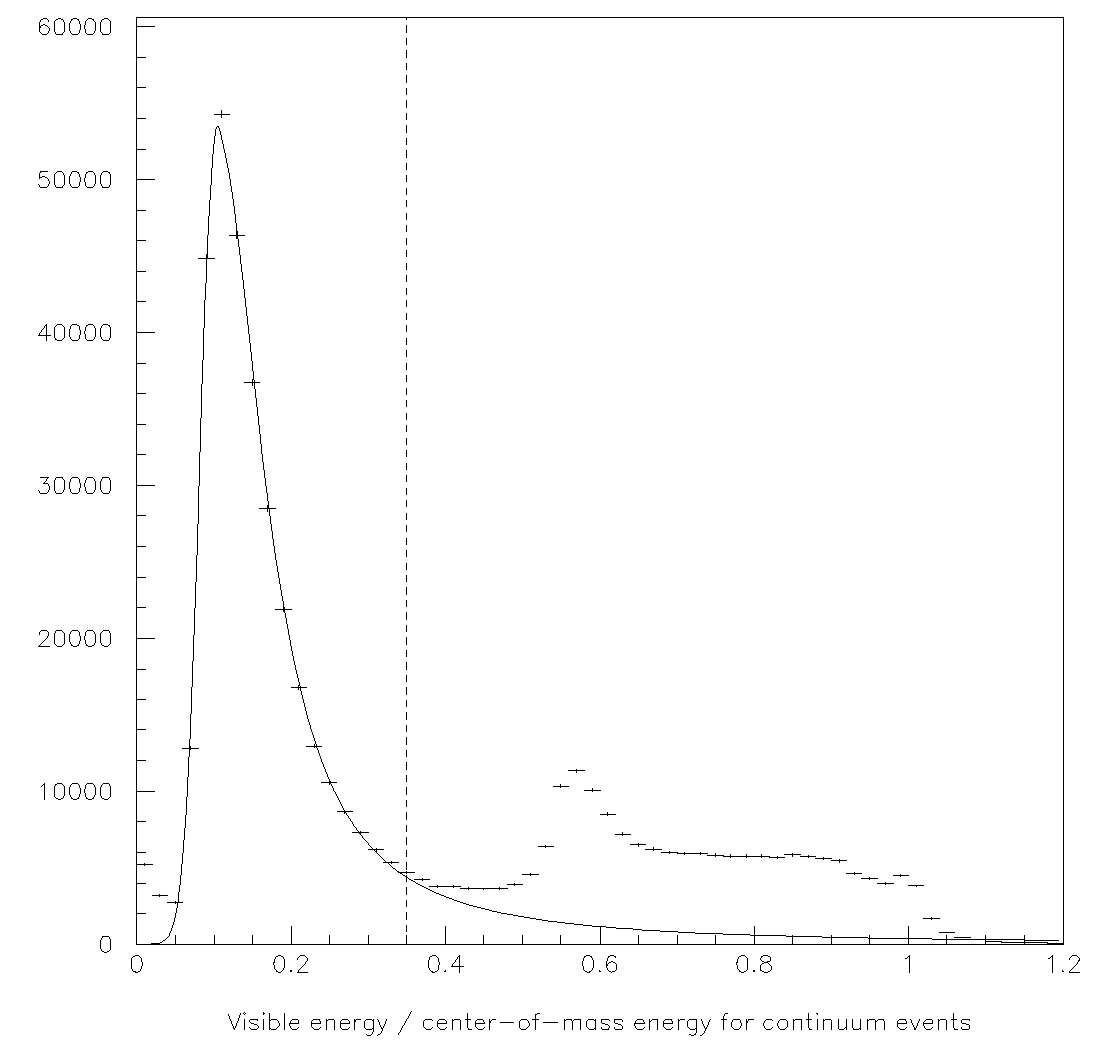
\includegraphics[width=0.7\linewidth]{twophoton_leakage.pdf}

After cut: 6\% of continuum is two-photon.  $1/s$ versus $\log s$
correction is a $\frac{1}{2}$\% correction to continuum scale factor.
Propogating this scale factor uncertainty after all cuts: 0.01\%,
0.03\%, 0.04\% two-photon contamination in continuum-subtracted
$\Upsilon$ dataset.

\pagebreak

In detailed studies, surviving non-beam-beam is -0.05\%, -0.11\%,
-0.27\%, but this is from a subsample of the data.  What about all
data?

\vfill
BEFORE continuum subtraction (some of these runs are continuum):

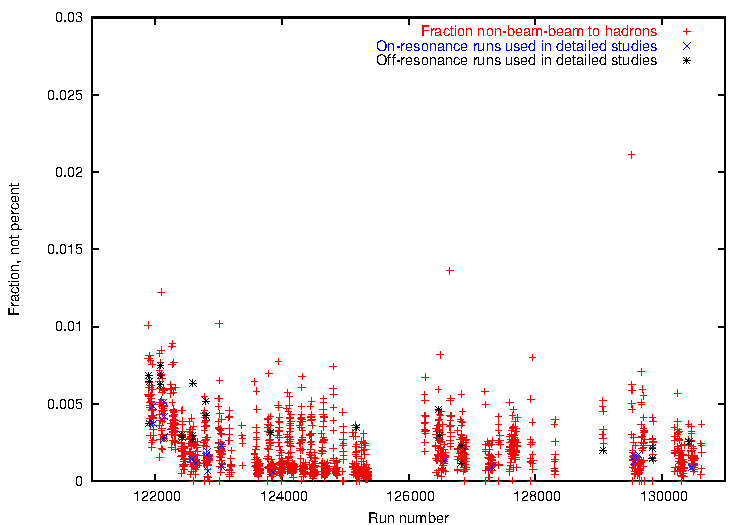
\includegraphics[width=0.7\linewidth]{non-beam-beam.pdf}

\pagebreak

The same thing histogrammed:

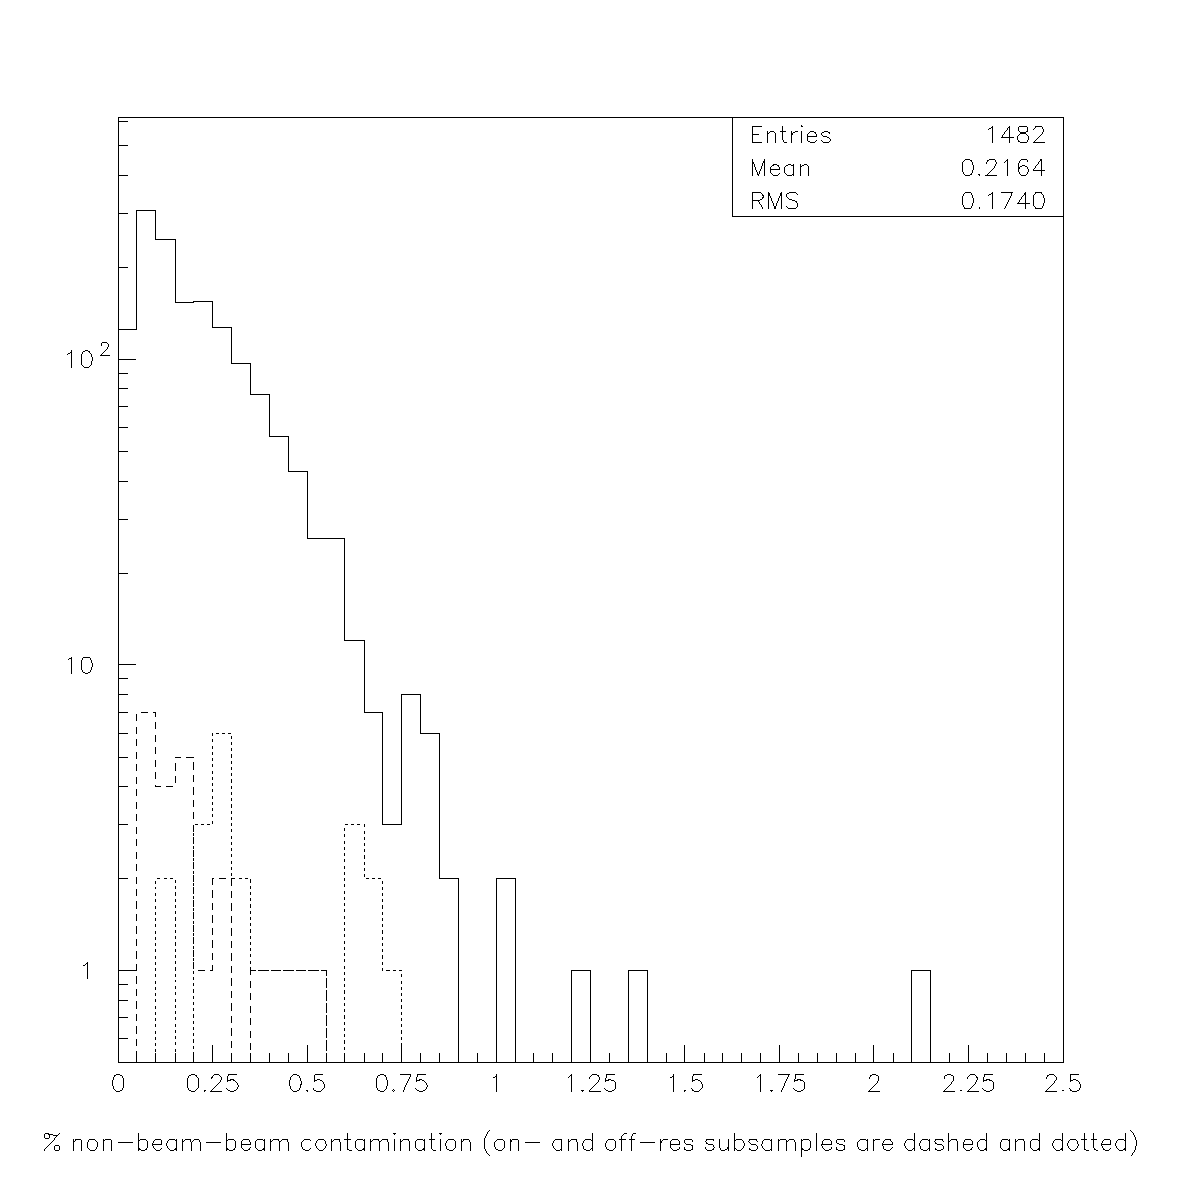
\includegraphics[width=0.7\linewidth]{hist_nbb.pdf}

Biggest scan contamination: 1.0\% (next is 0.8\%\ldots)

Add up ALL on-, off-resonance, do continuum subtraction, remaining
non-beam-beam background is -0.0029 nb, -0.00068 nb, -0.0025 nb.

\pagebreak

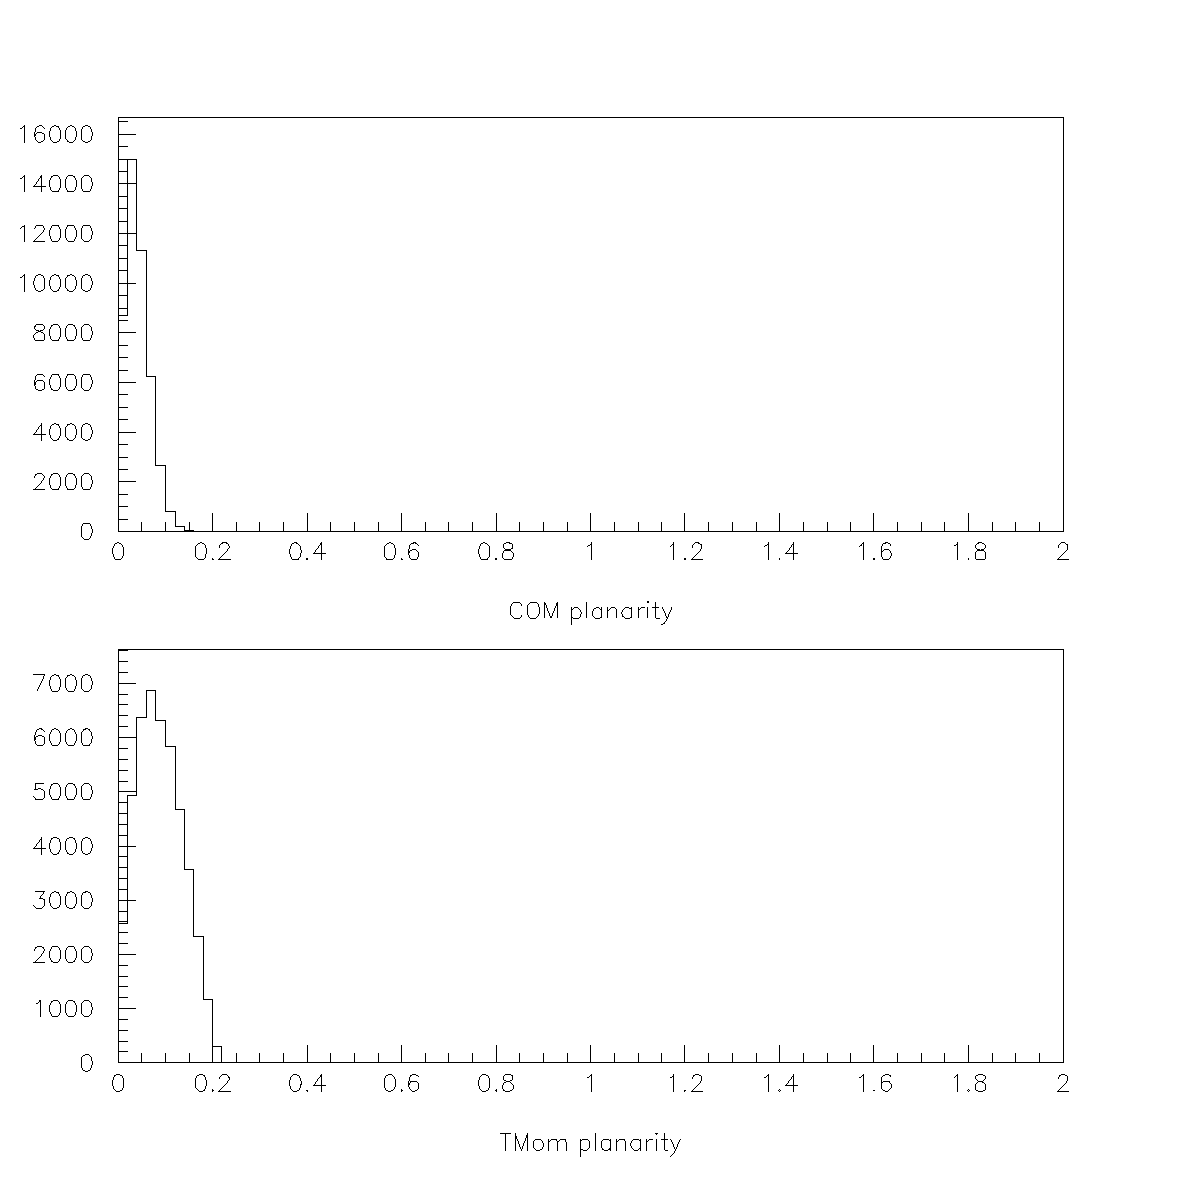
\includegraphics[width=0.7\linewidth]{lookatmc1.pdf}

(Generator-level planarity)

\pagebreak

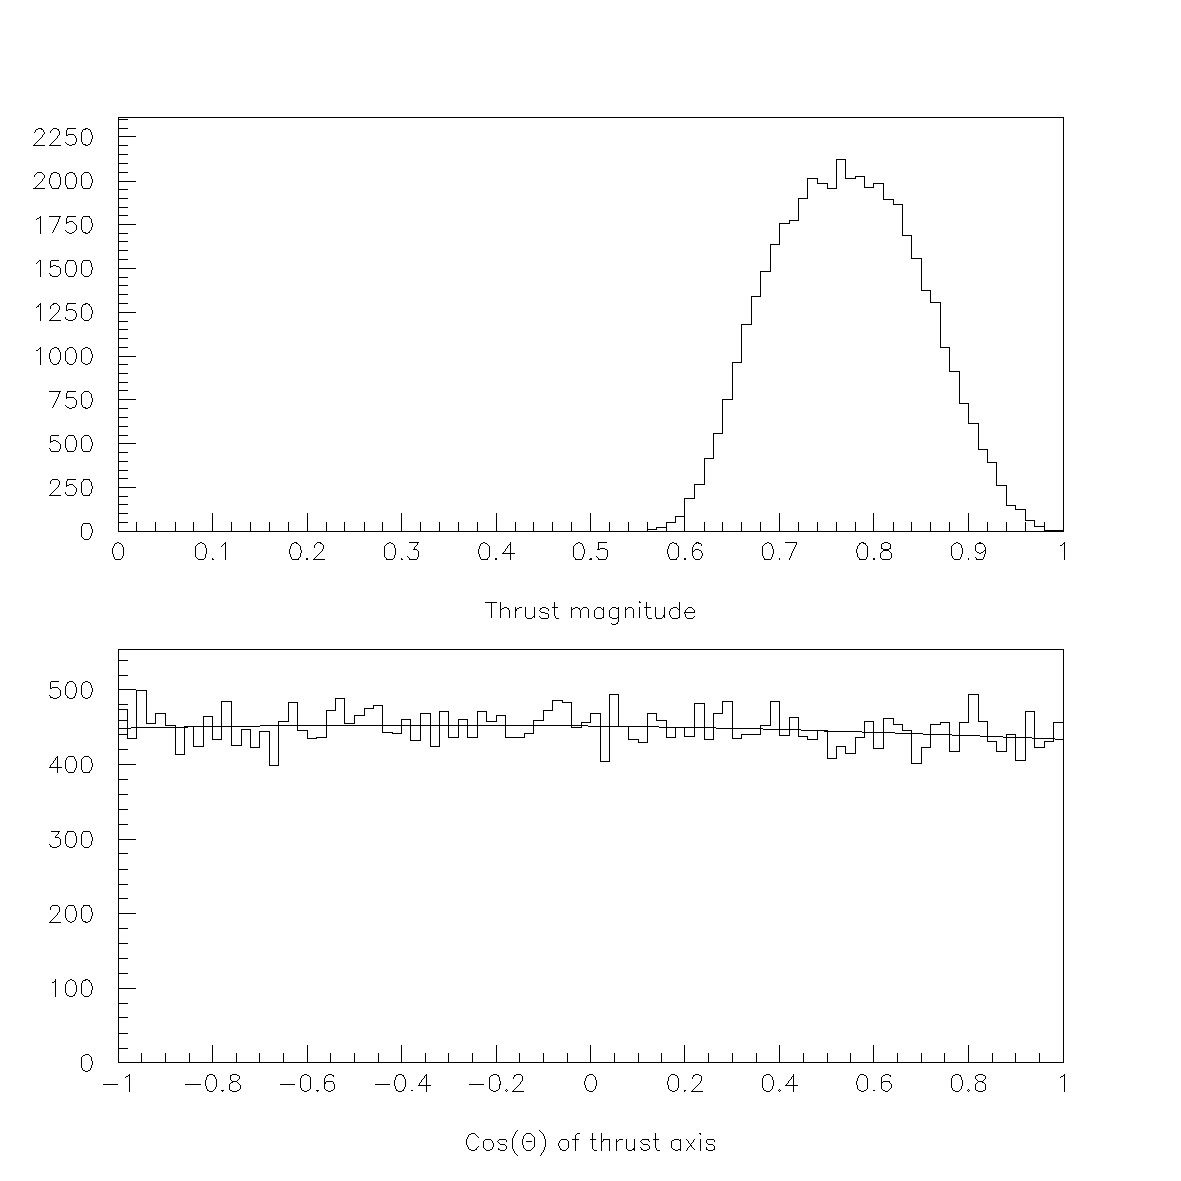
\includegraphics[width=0.7\linewidth]{lookatmc2.pdf}

Hadronized thrust axis (generator level) is $1 - 0.023(\pm 0.016)
\cos^2\theta$: consistent with being flat.  Looking for $+0.32$,
violated by 20$\sigma$.

\end{document}
